% Paper 1 (QEC-SB) -- target: IEEE Transactions on Quantum Engineering
% Compile: pdflatex main && bibtex main && pdflatex main && pdflatex main   (or Overleaf, IEEEtran is built in)
% Figures: paper/figures/*.pdf are produced by  python analysis/make_paper_figures.py
%          if a PDF is missing, the older analysis PNG in figures/fallback/ is used instead.
\documentclass[journal]{IEEEtran}

\usepackage[T1]{fontenc}
\usepackage{amsmath,amssymb,amsfonts}
\usepackage{graphicx}
\usepackage{booktabs}
\usepackage{multirow}
\usepackage{xcolor}
\usepackage{tikz}
\usetikzlibrary{arrows.meta,positioning,fit,calc}
\usepackage{algorithm}
\usepackage{algpseudocode}
\usepackage{url}
\usepackage[hidelinks]{hyperref}
\usepackage[capitalise,nameinlink]{cleveref}

\newcommand{\todo}[1]{\textcolor{red}{[TODO: #1]}}
\newcommand{\REF}{\mathrm{REF}}
\newcommand{\LER}{\mathrm{LER}}
\newcommand{\F}{\mathbb{F}_2}
\newcommand{\fig}[2]{\IfFileExists{figures/#1.pdf}{\includegraphics[width=#2]{figures/#1.pdf}}{\includegraphics[width=#2]{figures/fallback/#1.png}}}

\begin{document}

\title{Constraint-Preserving Simulated Bifurcation with Local Degeneracy Aggregation: How Close to Maximum-Likelihood Surface-Code Decoding?}

\author{Yaocheng~Chen and JiaPei~\todo{surname}%
\thanks{Y.~Chen is with the Instituto de Astronomia, Geof\'isica e Ci\^encias Atmosf\'ericas, Universidade de S\~ao Paulo, S\~ao Paulo, Brazil (e-mail: yaochengchen@iag.usp.br).}%
\thanks{JiaPei \todo{affiliation}.}%
\thanks{Y.~Chen acknowledges support from FAPESP \todo{grant number}.}}

\markboth{IEEE Transactions on Quantum Engineering}{Chen \MakeLowercase{\textit{et al.}}: Constraint-preserving SB decoding}

\maketitle

\begin{abstract}
Maximum-likelihood (ML) decoding of a stabilizer code selects the logical class with the largest total probability, whereas Ising-machine decoders usually return a single minimum-weight configuration. We study a decoder that separates the two tasks. A discrete simulated-bifurcation (SB) dynamics searches each logical class in stabilizer-generator coordinates, so that every state it visits is syndrome-feasible, and a local stabilizer-orbit expansion (SOE) around the best candidate of each class estimates the class probability. We benchmark the decoder on the rotated surface code under code-capacity depolarizing noise against exact ML ($d=3$) and a matrix-product-state (MPS) near-ML reference. After fixing the method on a separate selection set, we evaluate it on a held-out grid of 54 cells ($d=3$--$13$, $p=0.04$--$0.18$, $7.1\times10^{6}$ paired shots). The decoder beats minimum-weight perfect matching and a correlated BP+OSD baseline in all 54 cells after Holm correction. For $d\le 9$ its logical error rate is within $1.15\times$ of the reference everywhere and statistically indistinguishable from it in 27 of the 36 cells. With the search budget frozen at the value tuned for small codes, accuracy degrades at $d\ge 11$ and the $d=11/13$ crossing falls to $p\approx0.11$. Lengthening the bifurcation sweep fourfold reduces the ratio to the reference to $1.07$--$1.23$ and moves the crossing to $p\approx0.16$ (reference: $0.175$). A budget study shows that the sweep length, not the number of replicas, is the resource that must grow with $d$; that SB and a constraint-preserving simulated-annealing baseline reach the same accuracy plateau, SB in $42$--$84\times$ fewer sequential update rounds at $2$--$4\times$ more single-flip energy evaluations; and that the remaining excess (at most $13\%$ at the largest budgets) is set by the locality of the degeneracy estimate rather than by the search. On this planar benchmark the MPS decoder remains more accurate at a comparable CPU time; the proposed decoder requires only a stabilizer generator matrix, and the benchmark measures how far such a generic decoder is from ML.
\end{abstract}

\begin{IEEEkeywords}
Quantum error correction, surface code, maximum-likelihood decoding, degeneracy, simulated bifurcation, Ising machines, simulated annealing.
\end{IEEEkeywords}

% =====================================================================
\section{Introduction}
\label{sec:intro}

\IEEEPARstart{A}{} decoder for a stabilizer code receives a syndrome and must return a correction whose product with the actual error is a stabilizer. Because many physical errors share the same syndrome and differ only by stabilizers, the quantity that determines success is the total probability of each \emph{logical class} of errors, not the probability of any single error~\cite{dennis2002}. Maximum-likelihood decoding (MLD) chooses the class with the largest total probability; minimum-weight decoding chooses the class containing the single most probable error. The two differ precisely when degeneracy matters, and the difference grows with the code distance $d$ and the physical error rate $p$.

Exact MLD is \#P-hard in general~\cite{iyer2015}. For the planar surface code, tensor-network contraction with a matrix-product-state (MPS) boundary~\cite{bravyi2014} gives a controlled approximation that is essentially exact at moderate bond dimension; generalizations exist for two-dimensional local codes~\cite{darmawan2018,chubb2021}. Monte Carlo methods estimate class probabilities by sampling~\cite{wootton2012,hutter2014,martinezgarcia2024,tobias2026}. Matching~\cite{edmonds1965,higgott2022,higgott2025} and belief propagation with ordered-statistics post-processing (BP+OSD)~\cite{panteleev2021,roffe2020} are fast but ignore part of the degeneracy and, under depolarizing noise, the correlation between $X$ and $Z$ components.

A separate line of work maps decoding onto an Ising problem solved by an annealer or an Ising machine~\cite{fujisaki2022,fujisaki2023,takeuchi2023,takada2024}. Writing the error as a fixed syndrome-compatible seed times a product of stabilizer generators makes every spin configuration syndrome-feasible~\cite{takeuchi2023,takada2024}; the objective is then the Pauli weight, a low-order polynomial of the generator spins. These decoders return a minimum-weight solution and therefore, by construction, do not perform MLD.

Simulated bifurcation (SB)~\cite{goto2019,goto2021} is a deterministic, synchronously updated dynamical system for Ising problems. Its update is a matrix--vector-type operation applied to all variables and replicas at once, which makes it attractive for parallel hardware. To our knowledge SB has not been studied as a quantum decoder.

In this paper we combine SB search in stabilizer coordinates with a cheap estimate of each class's probability mass, and we ask how close the result comes to MLD as the code grows. Our contributions are:

\begin{enumerate}
\item A decoder (CP-SB + local SOE, \cref{sec:method}) that runs discrete SB on the exact Pauli-weight polynomial of each logical class and then aggregates the probability of all errors within a small Hamming radius, in generator space, of the best candidate of each class.
\item A two-stage evaluation (\cref{sec:protocol}) in which the method is fixed on a selection set by a rule stated in advance and then tested on a held-out $54$-cell grid ($d=3$--$13$) against exact MLD and an MPS reference, with paired tests against matching, correlated BP+OSD, and a constraint-preserving simulated-annealing (CP-SA) twin that shares everything but the search dynamics.
\item A decomposition of the remaining gap to ML (\cref{sec:results}): how much is due to the search (budget), how much to degeneracy that a minimum-weight decision misses, and how much to the locality of the degeneracy estimate. In particular, the sweep length of the bifurcation, not the number of parallel replicas, must grow with $d$.
\end{enumerate}

We state the limits of the result up front. All experiments use code-capacity noise on the planar rotated surface code, where an MPS decoder gives reference-quality decisions at a cost comparable to ours on a CPU (\cref{sec:cost}). We chose this benchmark because it is the setting in which a near-exact reference exists for $d$ up to 13, so that the distance to ML can be measured rather than inferred. The value of the proposed decoder is that its two ingredients need only a stabilizer generator matrix and a Pauli-weight oracle; testing it on codes without planar structure, and on hardware, is left to future work.

% =====================================================================
\section{Background and related work}
\label{sec:related}

\subsection{Degeneracy and maximum-likelihood decoding}
Let $e\in\F^{2n}$ denote an $n$-qubit Pauli error in binary symplectic form and $|e|$ its weight (number of non-identity qubits). Under depolarizing noise each qubit independently suffers $X$, $Y$, or $Z$ with probability $p/3$ each, so
\begin{equation}
\Pr(e)\propto w^{|e|},\qquad w=\frac{p/3}{1-p}.
\end{equation}
Given the syndrome $s$, choose any error $e_0$ with syndrome $s$, and let $\ell_L$ ($L=0,\dots,3$) be representatives of the four logical cosets. With $G\in\F^{m\times 2n}$ a generator matrix of the stabilizer group, the class-$L$ probability is
\begin{equation}
Z_L(s)=\sum_{u\in\F^m} w^{\,|e_0\oplus \ell_L\oplus uG|}.
\label{eq:ZL}
\end{equation}
MLD returns $\arg\max_L Z_L$; minimum-weight (MAP) decoding returns the class of $\arg\min_{L,u}|e_0\oplus\ell_L\oplus uG|$. Recent work shows that for planar surface codes the two decisions already differ at error weight $\lceil d/2\rceil$, i.e., at leading order~\cite{zhao2026}; degeneracy is therefore not a high-$p$ curiosity on this code.

\subsection{Near-ML decoders}
The MPS decoder of Bravyi, Suchara and Vargo contracts the planar tensor network of \cref{eq:ZL} with bond dimension $\chi$~\cite{bravyi2014}; it is exact as $\chi\to\infty$ and in practice converges at small $\chi$. Markov-chain Monte Carlo over the stabilizer group~\cite{wootton2012,hutter2014}, population annealing~\cite{martinezgarcia2024}, worm algorithms~\cite{tobias2026}, and annealed importance sampling with certificates~\cite{krishnamoorthy2026} estimate $Z_L$ or ratios of $Z_L$. Closest to our aggregation step, Liu \emph{et al.}~\cite{liu2026amld} recycle the candidates produced by a stochastic inner decoder into a truncated free energy per class. Our SOE differs in that it does not use the raw candidate pool as the sum: it enumerates a complete Hamming ball in generator space around the single best candidate of each class (\cref{sec:soe}), which recovers degenerate neighbors that the solver never visits.

\subsection{Ising-machine decoders}
Fujisaki \emph{et al.} formulated surface-code decoding as a QUBO with syndrome penalties and solved it on a digital annealer, including circuit-level noise~\cite{fujisaki2022,fujisaki2023}. Takeuchi \emph{et al.}~\cite{takeuchi2023} and Takada \emph{et al.}~\cite{takada2024} replaced the penalty by stabilizer-generator variables, so that every configuration is feasible, and used simulated annealing~\cite{kirkpatrick1983}. We adopt the same constraint-preserving coordinates; we do not claim them as new. What we add is SB as the search dynamics, an explicit degeneracy-aware decision, and a quantitative comparison with ML.

\subsection{Simulated bifurcation}
SB integrates a classical Hamiltonian system whose position variables undergo a pitchfork bifurcation as a control parameter is ramped, so that their signs settle into a low-energy Ising configuration~\cite{goto2019}. The ballistic and discrete variants (bSB, dSB) add inelastic walls at $|x|=1$; dSB evaluates the interaction on the signs of the positions~\cite{goto2021}. We use a dSB-type update with the exact multilinear force of a higher-order (up to four-body) polynomial.

% =====================================================================
\section{Method}
\label{sec:method}

\begin{figure}[t]
\centering
\resizebox{\columnwidth}{!}{%
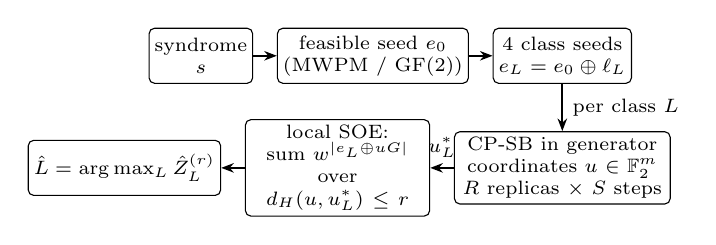
\begin{tikzpicture}[font=\scriptsize, node distance=3.5mm and 3mm,
  box/.style={draw, rounded corners=2pt, align=center, minimum height=7mm, inner sep=2pt, fill=white},
  arr/.style={-{Stealth[length=1.6mm]}, thick}]
\node[box] (s) {syndrome\\$s$};
\node[box, right=of s] (seed) {feasible seed $e_0$\\(MWPM / GF(2))};
\node[box, right=of seed] (cls) {4 class seeds\\$e_L=e_0\oplus\ell_L$};
\node[box, below=6mm of cls, text width=26mm] (sb) {CP-SB in generator\\coordinates $u\in\F^{m}$\\$R$ replicas $\times$ $S$ steps};
\node[box, left=of sb, text width=22mm] (soe) {local SOE: sum $w^{|e_L\oplus uG|}$\\over $d_H(u,u_L^\ast)\le r$};
\node[box, left=of soe] (dec) {$\hat L=\arg\max_L \hat Z_L^{(r)}$};
\draw[arr] (s) -- (seed);
\draw[arr] (seed) -- (cls);
\draw[arr] (cls) -- node[right, align=left]{per class $L$} (sb);
\draw[arr] (sb) -- node[above]{$u_L^\ast$} (soe);
\draw[arr] (soe) -- (dec);
\end{tikzpicture}}
\caption{Decoder pipeline. Every state visited by the search is syndrome-feasible because the search runs in stabilizer-generator coordinates. The search supplies the best candidate $u_L^\ast$ of each class; the local stabilizer-orbit expansion (SOE) supplies an estimate of the class probability $Z_L$.}
\label{fig:pipeline}
\end{figure}

\subsection{Code, noise and feasible seed}
We use the rotated surface code~\cite{bombin2007,fowler2012} with $n=d^2$ data qubits and $m=d^2-1$ independent stabilizer generators ($(d^2-1)/2$ of each type), and code-capacity depolarizing noise at rate $p$. A feasible correction $e_0$ is obtained from minimum-weight perfect matching (MWPM) applied separately to the $X$ and $Z$ components (any GF(2) solution would do); the four class seeds are $e_L=e_0\oplus\ell_L$ (\cref{fig:pipeline}).

\subsection{Pauli-weight Hamiltonian in generator coordinates}
For class $L$ every error is $e_L(u)=e_L\oplus uG$ with $u\in\F^m$. With spins $\sigma_j=(-1)^{u_j}$, the indicator that qubit $q$ carries a non-identity Pauli is
\begin{equation}
\mathbb{1}[e_q\neq I]=\tfrac34-\tfrac14\tau^x_q-\tfrac14\tau^z_q-\tfrac14\tau^x_q\tau^z_q,
\end{equation}
where $\tau^x_q=(-1)^{(e_L)^x_q}\prod_{j\in\mathcal{X}(q)}\sigma_j$ and $\mathcal{X}(q)$ is the set of generators whose $X$ part acts on $q$ (similarly for $z$). Summing over $q$ gives the energy $E_L(\sigma)=|e_L(u)|$ exactly, as a multilinear polynomial. On the rotated surface code each qubit is touched by at most two generators of each type, so $E_L$ has terms of order at most four, and there is no penalty term and no auxiliary spin. Because $\Pr(e)\propto w^{|e|}$, minimizing $E_L$ is MAP decoding within class $L$.

\subsection{Constraint-preserving SB (CP-SB)}
\label{sec:cpsb}
For each class we evolve $R$ replicas of positions $x\in[-1,1]^m$ and momenta $y\in\mathbb{R}^m$ for $S$ steps:
\begin{align}
y &\leftarrow y + \Delta t\,\bigl[-(1-a_k)\,x + c\, f(\operatorname{sgn} x)\bigr],\\
x &\leftarrow x + \Delta t\, y,
\end{align}
followed by inelastic walls ($x_j\leftarrow\operatorname{sgn}x_j$, $y_j\leftarrow0$ whenever $|x_j|>1$). The control parameter ramps linearly, $a_k=(k+1)/S$. The force is the exact negative gradient of the multilinear energy at the sign vertex, which we compute from single-generator flip energies:
\begin{equation}
f_j(\sigma)=-\frac{\partial E_L}{\partial\sigma_j}=\tfrac12\,\sigma_j\,\bigl[E_L(\sigma^{(j)})-E_L(\sigma)\bigr],
\end{equation}
where $\sigma^{(j)}$ is $\sigma$ with spin $j$ flipped. The coupling is normalized per class, $c=\kappa/\max_j B_j$ with $B_j$ the $\ell_1$ norm of the coefficients of all monomials containing $j$. Each class receives one \emph{warm} restart, initialized near the seed ($x=0.08+\mathcal{N}(0,0.01^2)$, i.e., $u=0$), and one \emph{random} restart ($x\sim\mathcal{U}(-0.1,0.1)$), each with $R$ replicas. The terminal sign vectors, together with $u=0$, form the candidate pool of the class. We denote a budget by $R\times S$; the frozen setting is $8\times100$ with $\Delta t=0.45$ and $\kappa=0.70$, fixed during earlier development on $d\le 9$. A decode therefore runs $4\times2\times R$ trajectories of $S$ steps.

\subsection{Local stabilizer-orbit expansion (SOE)}
\label{sec:soe}
Let $u_L^\ast$ be the lowest-energy candidate of class $L$. For radius $r$ we enumerate the Hamming ball $\mathcal{B}_r(u_L^\ast)=\{u: d_H(u,u_L^\ast)\le r\}$ in generator space---all products of at most $r$ generators applied to the best candidate---and estimate
\begin{equation}
\hat Z_L^{(r)}=\sum_{u\in\mathcal{B}_r(u_L^\ast)} w^{E_L(u)},\qquad \hat L=\arg\max_L \hat Z_L^{(r)}.
\label{eq:soe}
\end{equation}
$\hat Z_L^{(r)}$ is a lower bound on $Z_L$ that contains the dominant local degenerate neighbors of the best error. The ball has $1+m$ states for $r=1$ and $1+m+\binom{m}{2}$ for $r=2$ ($169$ and $14{,}197$ per class at $d=13$), but the sum does not require enumerating the ball. The Pauli weight is a sum over qubits, so flipping two generators with disjoint qubit supports changes $E_L$ by the sum of the two single-flip changes $\Delta_j=E_L(u_L^\ast\oplus\mathbf{e}_j)-E_L(u_L^\ast)$. The number of ball states at each weight is therefore the self-convolution of the histogram of the $m$ values $\Delta_j$ (minus the $j=k$ terms), corrected only on the pairs of generators whose supports overlap---at most eight per generator on the rotated surface code, $O(m)$ pairs in total---for which the true change is computed directly. This evaluates \cref{eq:soe} exactly, in integer arithmetic, at $O(m)$ cost for $r=2$, and uses nothing but the supports of the rows of $G$. SOE needs no sampling and no tuning beyond $r$; its cost is independent of the search budget. Heavier mass estimators that we tried earlier---adaptive importance sampling and a Bennett acceptance-ratio refinement---did not improve on $r=2$ on the held-out grid (median $\LER/\LER_\REF$ $1.040$ and $1.054$ versus $1.039$) and are not discussed further.

\subsection{CP-SA twin}
To separate the effect of the search dynamics from everything else, we use a constraint-preserving simulated-annealing twin (CP-SA) that shares the seeds, the Hamiltonian, the pool construction and the SOE step. It performs single-generator Metropolis flips with a geometric temperature schedule from $2.0$ to $0.05$ over $W$ sweeps, with $C$ chains for each of the warm and random modes; we denote its budget by $C\times W$ (grid setting $8\times100$).

% =====================================================================
\section{Experimental protocol}
\label{sec:protocol}

\subsection{Two-stage design}
\emph{Selection set.} $12{,}000$ shots at $d=5,7,9$ and $p=0.10,0.12$ ($3000$, $2000$ and $1000$ shots per cell). Before the held-out data existed we fixed the rule: the main decoder is CP-SB + SOE with $r=1$, replaced by $r=2$ only if $r=2$ has strictly fewer failures pooled over the selection set and an exact paired McNemar test gives $p<0.05$. Radius 2 won ($70$ shots corrected that $r=1$ missed versus $40$ the other way, $p=0.0054$), so the main decoder is \textbf{CP-SB $8\times100$ + SOE $r=2$}.

\emph{Held-out grid.} $54$ cells, $d\in\{3,5,7,9,11,13\}$, $p\in\{0.04,0.05,0.06,0.08,0.10,0.12,0.14,0.16,0.18\}$, with seeds disjoint from the selection set. Shots per cell range from $10^4$ ($p\ge0.14$) to $10^6$ ($d\ge11$, $p=0.04$), $7.12\times10^6$ in total; every decoder decodes the same shots, so all comparisons are paired. The full per-cell table is in \cref{app:table}.

\subsection{Baselines}
(i) MWPM on the $X$ and $Z$ components with unit weights; PyMatching~\cite{higgott2022} with $p$-dependent weights gave identical predictions on every grid shot, and we report them together. (ii) BP+OSD-CS~\cite{panteleev2021,roffe2020} (order 7, min-sum, \texttt{ldpc}~\cite{ldpc}), first on the $X$ and $Z$ components separately with prior $2p/3$, and (iii) a \emph{correlated} version on the matrix $\bigl[\begin{smallmatrix}H_Z & 0 & H_Z\\ 0 & H_X & H_X\end{smallmatrix}\bigr]$ whose three column blocks are the $X$, $Z$ and $Y$ components, each with prior $p/3$ and $3n$ iterations. The correlated version is better than the independent one in all 54 cells (Holm $p\le 0.0014$; at $d=13$, $p=0.10$ its $\LER/\LER_\REF$ is $2.67$ instead of $5.14$), so it is the BP baseline we report. (iv) CP-SA with the same SOE.

\subsection{Reference and its validation}
The reference (REF) is exact MLD at $d=3$ (enumeration of the $2^8$ stabilizer group per class), MPS with $\chi=32$ for $d=5$--$9$~\cite{bravyi2014,qecsim}, and MPS with $\chi=16$ for $d=11,13$, replaced by $\chi=32$ on every \emph{hard} shot (any decoder wrong or disagreeing with $\chi=16$; up to 3000 per cell). Checks: at $d=3$ the MPS decisions agree with exact MLD on $100\%$ of non-tied syndromes ($4695$ and $4610$ shots at $p=0.10,0.12$). On the grid, $\chi=16$ and $\chi=32$ disagree on at most 7 shots per cell at $d=9$ and at most 2 hard shots per cell at $d\ge11$; on the $d\ge11$ hard shots $\chi=32$ and $\chi=64$ disagree on at most 1 shot per cell (18 cells, 401--3000 shots each). At $d=5$ the $\chi=16/32$ disagreements are more frequent (67--188 per cell), but they are near-ties and vanish at larger $d$; we use $\chi=32$ there.

\subsection{Metrics and statistics}
We report the logical error rate (LER) with Wilson 95\% intervals, the ratio $\LER/\LER_\REF$, and the gap closure relative to MWPM,
\begin{equation}
G=\frac{\LER_{\mathrm{MWPM}}-\LER_X}{\LER_{\mathrm{MWPM}}-\LER_\REF},
\end{equation}
with a paired bootstrap interval. Paired comparisons use the exact two-sided McNemar (sign) test on discordant shots, Holm-corrected across all cells of a comparison family. Where per-cell tests are underpowered we also report the discordant counts pooled over cells with an exact sign test; we treat these pooled tests as descriptive.

\subsection{Budget study and budget-scaled rows}
\label{sec:budgetprotocol}
On the first $10^4$ shots of every cell with $d\in\{9,11,13\}$ and $p=0.08$--$0.16$ we decoded with CP-SB budgets $R\times S\in\{8\times100,16\times100,32\times100,64\times100,8\times200,8\times400,32\times400\}$ and CP-SA budgets $C\times W\in\{8\times25,8\times50,8\times100,8\times200,16\times100,32\times200\}$, each with MAP, SOE $r=1$ and SOE $r=2$ decisions; at $p=0.18$ we ran five of these configurations. The $8\times100$ configurations reproduce the grid decisions shot by shot. From this study we then fixed a single rule---keep $R=8$ and use $S=400$ for $d\ge11$---and applied it to the full grid cells at $d=11,13$ (all shots for $p\ge0.08$, the first $10^5$ shots for $p\le0.06$). Because the rule was chosen after the budget study, and at $p\ge0.14$ the study used the same shots, we present these \emph{budget-scaled} rows as a budget study next to the frozen held-out rows, not as an independent confirmation.

\subsection{Timing}
Times are single-process CPU wall times per unique non-trivial syndrome on an otherwise idle node (AMD EPYC 9754; Python 3.11, NumPy 2.4), medians over 100 unique syndromes at $p=0.10$ for $d\ge 7$, for every decoder and budget configuration. An earlier run at $p=0.14$ gave medians within a few percent of those at $p=0.10$. Both searches compute the energy change of a generator flip from the at most four qubits the generator touches: CP-SB evaluates all $m$ flips of all replicas in one batched NumPy operation per step, whereas CP-SA evaluates one flip at a time in a Python loop, as the sequential Metropolis rule requires; SOE uses the histogram evaluation of \cref{sec:soe}. The CP times come from one run on the same syndromes, which also times our earlier full-vector flip evaluation and the explicit enumeration of the SOE ball; both give identical candidate pools and decisions. PyMatching (compiled C++), BP+OSD (Cython) and the MPS decoder (the Python implementation in \texttt{qecsim}~\cite{qecsim}) were timed in an earlier run on the same cluster; the full-vector CP-SB and CP-SA search times of that run are reproduced by the new one to within $2\%$. Because wall times depend on such implementation choices, we also report two implementation-independent counts per decode: the number of single-flip energy evaluations ($8RSm$ for CP-SB, $8CWm$ for CP-SA: four classes, two restart modes) and the number of sequential update rounds ($S$ for CP-SB, whose steps update all variables and replicas at once; $Wm$ for CP-SA). Times therefore describe this benchmark, not hardware limits.

% =====================================================================
\section{Results}
\label{sec:results}

\begin{figure*}[t]
\centering
\fig{fig_ratio_vs_p}{\textwidth}
\caption{Logical error rate relative to the reference on the held-out grid. Dotted line: reference (exact MLD at $d=3$, MPS otherwise). Dashed: the budget-scaled CP-SB $8\times400$ + SOE $r=2$ at $d\ge11$ (\cref{sec:budget}). At $d=11,13$ and $p\le0.06$ the reference has fewer than 100 failures per cell and the ratios are noisy.}
\label{fig:ratio}
\end{figure*}

\begin{table}[t]
\centering
\caption{$\LER/\LER_\REF$ on the held-out grid (selected cells; all 54 in \cref{app:table}). REF in percent. $^{*}$: significantly worse than REF (Holm $p<0.05$). The last column is the budget-scaled $8\times400$ row (\cref{sec:budget}).}
\label{tab:main}
\footnotesize
\setlength{\tabcolsep}{3.2pt}
\resizebox{\columnwidth}{!}{%
\begin{tabular}{rrrrrrrr}
\toprule
$d$ & $p$ & REF\,(\%) & MWPM & BP+OSD$_\mathrm{c}$ & SA+SOE$_1$ & SB+SOE$_2$ & SB$_{400}$+SOE$_2$\\
\midrule
3 & 0.08 & 6.99 & 1.13 & 1.05 & 1.00 & 1.01 & -- \\
3 & 0.12 & 13.8 & 1.11 & 1.05 & 1.00 & 1.01 & -- \\
3 & 0.16 & 21.8 & 1.09 & 1.04 & 0.99 & 0.99 & -- \\
\addlinespace
5 & 0.08 & 3.74 & 1.51 & 1.23 & 1.02 & 1.02 & -- \\
5 & 0.12 & 10.9 & 1.34 & 1.16 & 1.03 & 1.01 & -- \\
5 & 0.16 & 20.8 & 1.25 & 1.13 & 1.02 & 1.00 & -- \\
\addlinespace
7 & 0.08 & 1.94 & 2.04 & 1.53 & 1.04 & 1.04 & -- \\
7 & 0.12 & 7.74 & 1.71 & 1.44 & 1.07 & 1.06$^{*}$ & -- \\
7 & 0.16 & 18.7 & 1.46 & 1.34 & 1.07 & 1.06$^{*}$ & -- \\
\addlinespace
9 & 0.08 & 0.94 & 2.82 & 2.00 & 1.03 & 1.01 & -- \\
9 & 0.12 & 6.08 & 2.02 & 1.66 & 1.09 & 1.08$^{*}$ & -- \\
9 & 0.16 & 17.3 & 1.62 & 1.46 & 1.09 & 1.10$^{*}$ & -- \\
\addlinespace
11 & 0.08 & 0.50 & 3.97 & 2.68 & 1.07 & 1.20$^{*}$ & 1.10$^{*}$ \\
11 & 0.12 & 4.28 & 2.55 & 2.18 & 1.14 & 1.28$^{*}$ & 1.12$^{*}$ \\
11 & 0.16 & 16.3 & 1.73 & 1.60 & 1.11 & 1.22$^{*}$ & 1.10$^{*}$ \\
\addlinespace
13 & 0.08 & 0.23 & 5.74 & 3.99 & 1.23 & 1.87$^{*}$ & 1.07 \\
13 & 0.12 & 3.12 & 3.28 & 2.65 & 1.25 & 1.82$^{*}$ & 1.18$^{*}$ \\
13 & 0.16 & 15.1 & 1.93 & 1.88 & 1.25 & 1.54$^{*}$ & 1.19$^{*}$ \\
\bottomrule
\end{tabular}}
\end{table}

\subsection{Comparison with matching and BP+OSD}
The main decoder has a lower LER than MWPM/PyMatching and than correlated BP+OSD in all 54 cells, each significant after Holm correction (largest Holm $p$: $8.7\times10^{-12}$ against MWPM, $0.0077$ against correlated BP+OSD). Pooled over the grid, it corrects $55{,}081$ shots that MWPM fails on versus $17{,}007$ in the opposite direction, and $41{,}739$ versus $21{,}099$ against correlated BP+OSD. The margins grow with $d$ (\cref{fig:ratio}, \cref{tab:main}): at $d=13$, MWPM is $1.6$--$12\times$ and correlated BP+OSD $1.6$--$6.5\times$ the reference, compared with $1.3$--$1.9\times$ for our frozen decoder. Beating MWPM under depolarizing noise is expected of any decoder that uses the $X$--$Z$ correlation; the correlated BP+OSD comparison is the more informative one. No decoder lost effective distance: across the grid there is no failure of weight below $\lceil d/2\rceil$ except for independent BP+OSD (1--3 failures per cell at $d=9,11$, $p\le0.06$).

\subsection{Gap to ML at fixed budget}
\label{sec:gap}
For $d\le 9$ the frozen decoder is close to the reference: $\LER/\LER_\REF$ lies in $0.99$--$1.01$ at $d=3$, $1.00$--$1.04$ at $d=5$, $1.01$--$1.06$ at $d=7$ and $1.01$--$1.15$ at $d=9$; the gap closure is at least $0.85$ for $d\le7$ and at least $0.80$ at $d=9$. Across all 54 cells the paired test against the reference is not significant in 30 cells; the 24 significant cells (all in the direction of a higher LER for our decoder) are distributed as $0,1,2,6,7,8$ over $d=3,\dots,13$. At $d=11,13$ the frozen decoder degrades ($\LER/\LER_\REF$ up to $1.33$ and $1.87$), while the CP-SA twin at the same nominal budget stays at $1.06$--$1.14$ and $0.90$--$1.30$; CP-SA + SOE $r=1$ is significantly better than CP-SB + SOE $r=1$ in 15 cells, all of them at $d=11$ ($p\ge0.06$) or $d=13$ ($p\ge0.05$), and never the reverse. At this nominal budget both searches perform the same number of single-flip energy evaluations ($1.1\times10^6$ per decode at $d=13$), but the SB sweep has $100$ sequential rounds against $16{,}800$ for SA; as the next subsection shows, the gap closes when the SB sweep is lengthened.

The frozen budget also suppresses the threshold behavior. With $8\times100$, $\LER(d=13)$ exceeds $\LER(d=11)$ from $p=0.12$ on ($5.69\%$ vs $5.48\%$), a crossing at $p\approx0.11$; the reference curves for $d=11$ and $13$ cross at $p\approx0.175$ (\cref{fig:lervsd}).

\begin{figure*}[t]
\centering
\fig{fig_ler_vs_d}{\textwidth}
\caption{Logical error rate versus $d$ for each $p$. (a) Frozen budget CP-SB $8\times100$ + SOE $r=2$ at every $d$. (b) Same decoder with $S=400$ steps for $d\ge11$. (c) Reference. With the frozen budget the curves turn upward at $d=13$ already at $p\approx0.12$; with the longer sweep they decrease with $d$ up to $p=0.14$.}
\label{fig:lervsd}
\end{figure*}

\subsection{Scaling the search budget}
\label{sec:budget}
\emph{Budget-scaled rows.} Raising the number of SB steps from 100 to 400 at $d\ge11$ (replicas unchanged) lowers the LER in all 18 cells relative to the frozen decoder, significantly in 12 (Holm), all at $d=11$, $p\ge0.10$ or $d=13$, $p\ge0.06$; pooled, it corrects $6{,}429$ shots that the frozen decoder fails on versus $3{,}487$. For $p\ge0.08$, $\LER/\LER_\REF$ falls from $1.20$--$1.33$ to $1.09$--$1.12$ at $d=11$ and from $1.38$--$1.87$ to $1.07$--$1.23$ at $d=13$ (\cref{tab:main}, dashed lines in \cref{fig:ratio}). The budget-scaled rows remain significantly worse than the reference in 10 of 18 cells ($d=11$, $p\ge0.08$; $d=13$, $p\ge0.12$), by $9$--$23\%$.

\emph{Threshold.} With $8\times400$ the $d=11/13$ crossing moves from $p\approx0.11$ to $p\approx0.16$ ($\LER$ at $p=0.16$: $17.95\%$ vs $18.07\%$). In the budget study, CP-SB $32\times400$ and CP-SA $32\times200$ give LERs that decrease monotonically with $d$ up to $p=0.16$ (CP-SB $32\times400$ at $p=0.16$: $18.68$, $17.68$, $16.72\%$ for $d=9,11,13$) and cross between $0.16$ and $0.18$ ($p\approx0.17$), approaching the reference value $\approx0.175$. The low crossing of the frozen decoder is therefore a property of a budget that does not grow with $d$---CP-SA $8\times100$ also crosses early, between $p=0.14$ and $0.16$---and not a limit of the method. These finite-size crossings lie below the asymptotic optimal threshold of $\approx0.189$~\cite{bombin2012}, as expected at $d\le13$.

\begin{figure*}[t]
\centering
\fig{fig_budget}{\textwidth}
\caption{Budget study at $d=13$. Top: SOE $r=1$ accuracy versus search time per syndrome for CP-SB (blue) and CP-SA (orange); solid lines increase the number of steps (sweeps), dotted lines the number of replicas. Bottom: accuracy versus end-to-end time (seed + search + SOE) with $r=1$ and $r=2$ joined by a line; star: MPS $\chi=16$; diamond: correlated BP+OSD. Single-core median times at $p=0.10$ with the implementation of \cref{sec:protocol}; implementation-independent work counts are in \cref{tab:budget}.}
\label{fig:budget}
\end{figure*}

\emph{Steps versus replicas.} At equal work the longer sweep is better. At $d=13$, CP-SB $8\times400$ and $32\times100$ both perform $4.3\times10^6$ single-flip energy evaluations per decode; they give $\LER/\LER_\REF$ (SOE $r=2$, $p=0.10$--$0.16$) of $1.10$, $1.17$, $1.23$, $1.19$ and $1.23$, $1.28$, $1.33$, $1.29$; pooled over the 15 study cells, $8\times400$ corrects $1{,}935$ shots that $32\times100$ fails on versus $1{,}643$ (sign test $p\approx10^{-6}$; one cell significant on its own). $64\times100$, with twice the work, only matches $8\times400$ ($1{,}469$ vs $1{,}500$). Replicas are independent samples of the same quench: if the bifurcation is traversed too quickly for a given $m$, more replicas reproduce the same bias. A longer ramp lets the positions follow the slow bifurcation and settle into lower-energy sign patterns (\cref{fig:budget}, top).

\emph{SB versus SA.} When the decision rule is held fixed, the two searches converge to the same accuracy. Comparing budgets of similar accuracy, CP-SB $8\times400$ versus CP-SA $8\times100$ and CP-SB $32\times400$ versus CP-SA $32\times200$, none of the 18 cells is significant for any of MAP, SOE $r=1$ or SOE $r=2$, and the pooled discordant counts are balanced (SOE $r=2$: $3{,}169$ vs $3{,}048$ and $1{,}134$ vs $1{,}200$). The two searches spend their effort differently. At $d=13$, CP-SB $8\times400$ and $32\times400$ perform $4\times$ and $2\times$ as many single-flip energy evaluations as CP-SA $8\times100$ and $32\times200$ ($4.3$ vs $1.1$ and $17.2$ vs $8.6\times10^6$ per decode), but in $400$ sequential rounds instead of $16{,}800$ and $33{,}600$, i.e., $42\times$ and $84\times$ fewer (\cref{tab:budget}). In our single-core implementation the SB searches take $0.37$ and $0.84$\,s, the SA searches $1.08$ and $8.33$\,s; this wall-time ratio reflects a batched NumPy update against a Python loop as much as the two algorithms, which is why we base the comparison on the counts. The budget-scaled main decoder ($8\times400$, $r=2$) is not significantly different from the grid's CP-SA $8\times100$ + SOE $r=1$ in any of the 18 full cells either (pooled $3{,}265$ vs $2{,}914$, a small edge for SB). At low budget SB is clearly better: CP-SB $8\times100$ against CP-SA $8\times25$ ($1.1$ vs $0.27\times10^6$ evaluations, $100$ vs $4{,}200$ sequential rounds at $d=13$) is significant in 8 of 15 cells for SOE $r=1$, pooled $6{,}124$ vs $3{,}867$. We therefore claim the same accuracy plateau reached in far fewer sequential rounds, at the price of more total work; we do not claim a better plateau.

\subsection{Where the remaining gap comes from}
\label{sec:decomp}
\Cref{fig:decomp} decomposes the gap into search and degeneracy. The MAP decision (lowest-weight candidate over all classes) is $1.04$--$1.12\times$ the reference at $d=3$ and rises to $1.2$--$1.5\times$ at $d=9$ and $1.4$--$2.7\times$ at $d=13$ with the frozen budget. With a sufficient budget all searches return the same minimum-weight decision: at $d=13$, $p=0.12$ the MAP ratio is $1.37$--$1.38$ for CP-SA $8\times200$, $16\times100$, $32\times200$ and CP-SB $32\times400$. The remaining MAP excess is therefore not a search failure but degeneracy: the most probable single error lies in the wrong class. SOE recovers most of it---in the same cell SOE $r=2$ lowers the ratio from $1.38$ to $1.10$---and the share it recovers grows with $d$.

Radius 2 is better than radius 1 by a small, consistent margin. On the grid only 3 of 54 cells are individually significant, but 50 of 54 point the same way, and pooled over the grid $r=2$ corrects $5{,}222$ shots that $r=1$ misses versus $4{,}337$ ($p=1.5\times10^{-19}$). At $d=3$, where $r=1$ is already essentially MLD, the two are tied ($1{,}893$ vs $1{,}882$); every $d\ge5$ is significant on its own ($p<10^{-3}$). With the $8\times400$ search the picture is the same (0/18 cells, 12/18 in favor, pooled $569$ vs $376$).

At the largest budgets the ratio to the reference levels off independently of the search: SOE $r=2$ gives $1.05$--$1.08$ at $d=9$, $1.00$--$1.11$ at $d=11$ and $1.08$--$1.13$ at $d=13$ for $p\ge0.10$, for both CP-SB $32\times400$ and CP-SA $32\times200$. This plateau is the error of the local estimate \eqref{eq:soe} itself: the ball around a single center misses degenerate errors that differ from it by larger stabilizer products and the mass around other near-optimal centers. More search does not remove it; a larger or adaptive orbit would.

\begin{figure*}[t]
\centering
\fig{fig_decomposition}{\textwidth}
\caption{Gap decomposition on the held-out grid: minimum-weight decision of the search (MAP), plus SOE $r=1$, plus SOE $r=2$, all relative to the reference. Solid: frozen $8\times100$ search. Dashed, open markers ($d\ge11$): $8\times400$ search. The distance between MAP and SOE is the degeneracy that a minimum-weight decoder misses; the distance between SOE $r=2$ and 1 is the error of the local mass estimate.}
\label{fig:decomp}
\end{figure*}

\subsection{Cost}
\label{sec:cost}

\begin{table}[t]
\centering
\caption{Median single-core time per unique non-trivial syndrome at $p=0.10$ (seconds). 100 syndromes per entry. Python/NumPy as described in \cref{sec:protocol}, except PyMatching (C++) and BP+OSD (Cython). End-to-end times include the MWPM seed.}
\label{tab:time}
\footnotesize
\setlength{\tabcolsep}{4pt}
\resizebox{\columnwidth}{!}{%
\begin{tabular}{lrrr}
\toprule
 & $d=9$ & $d=11$ & $d=13$\\
\midrule
PyMatching & $2.7\times10^{-5}$ & $3.3\times10^{-5}$ & $4.3\times10^{-5}$\\
BP+OSD, correlated & $0.0011$ & $0.0025$ & $0.0050$\\
MPS $\chi=16$ & $0.164$ & $0.326$ & $0.540$\\
MPS $\chi=32$ & $0.659$ & $1.711$ & $3.269$\\
\midrule
CP-SB search $8\times100$ & $0.058$ & $0.077$ & $0.104$\\
CP-SB search $8\times400$ & $0.210$ & $0.275$ & $0.369$\\
CP-SB search $32\times400$ & $0.355$ & $0.528$ & $0.841$\\
CP-SA search $8\times100$ & $0.528$ & $0.780$ & $1.084$\\
CP-SA search $32\times200$ & $4.08$ & $6.09$ & $8.33$\\
SOE $r=2$, enumerating the ball & $0.258$ & $1.063$ & $3.540$\\
SOE $r=1$ & $3.7\times10^{-4}$ & $5.0\times10^{-4}$ & $7.0\times10^{-4}$\\
SOE $r=2$ & $4.6\times10^{-4}$ & $6.0\times10^{-4}$ & $8.2\times10^{-4}$\\
\midrule
End to end: $8\times100$ + SOE $r=2$ (frozen) & $0.060$ & $0.080$ & $0.110$\\
End to end: $8\times400$ + SOE $r=1$ & $0.212$ & $0.279$ & $0.375$\\
End to end: $8\times400$ + SOE $r=2$ & $0.212$ & $0.279$ & $0.375$\\
\bottomrule
\end{tabular}}
\end{table}

\Cref{tab:time} lists per-syndrome times. Two points matter for interpreting the results. First, the degeneracy estimate is negligible at both radii. Enumerating the $r=2$ ball explicitly costs $3.5$\,s at $d=13$; evaluated from the weight histogram (\cref{sec:soe}) the $r=2$ step takes $0.8$\,ms and $r=1$ $0.7$\,ms, a $4{,}300$-fold reduction for $r=2$. The two evaluations give the same class scores (largest relative difference $1.2\times10^{-15}$) and the same decision, for both radii, on all $42{,}800$ decodes of a consistency check ($d=3$--$13$, $p=0.06$, $0.10$, $0.14$, $0.18$; CP-SB $8\times100$, CP-SB $8\times400$ at $d\ge11$ and CP-SA $8\times100$ pools); the same check confirms that the sparse and full-vector flip evaluations produce identical candidate pools on every decode. The $1$--$3\%$ that $r=2$ gains over $r=1$ at $d=13$ therefore comes at no measurable cost, and the end-to-end time is set by the search: $0.11$\,s for the frozen decoder and $0.38$\,s for the budget-scaled one ($8\times400$ + SOE $r=2$) at $d=13$.

Second, on this benchmark the MPS decoder with $\chi=16$ reaches reference accuracy in $0.54$\,s at $d=13$ ($3.3$\,s with $\chi=32$). Our budget-scaled pipeline is somewhat faster in our single-core implementation ($0.38$\,s at $d=13$, $0.28$ versus $0.33$\,s at $d=11$) but stays $7$--$23\%$ above the reference, so neither decoder dominates the other on a planar code, and we do not claim that ours does. MPS contraction relies on the planar two-dimensional structure of the code; the two components of our decoder use only the generator matrix $G$ and the Pauli weight, and the dynamics is a synchronous update of all replicas and variables suited to parallel hardware. Neither of these properties is tested here (\cref{sec:discussion}).

\subsection{Reproducibility across solver seeds}
Three independent solver seeds for CP-SB $8\times100$ and CP-SA $8\times100$ (SOE $r=1$; $d=9,11,13$; $p=0.10,0.14$; $10^4$ shots each) give LERs within $0.06$--$0.54$ percentage points of each other. The fraction of shots on which all three seeds agree is $0.87$--$0.99$ for CP-SB and $0.90$--$0.99$ for CP-SA; the lower agreement of the frozen SB search at $d=13$, $p=0.14$ ($0.865$ vs $0.905$) is another sign that $8\times100$ does not converge there.

% =====================================================================
\section{Discussion}
\label{sec:discussion}

\emph{What the benchmark shows.} On the one code family where near-exact ML decisions are available up to $d=13$, a decoder made of a generic Ising search and a local degeneracy estimate comes within $1.15\times$ of ML for $d\le9$ and within $1.07$--$1.23\times$ at $d=11,13$ once its search budget grows with $d$. It beats correlated BP+OSD everywhere. The remaining excess separates cleanly into three parts: an undersized search budget (removed by longer SB sweeps), degeneracy that a minimum-weight decision misses (mostly recovered by SOE), and the locality of SOE (a plateau of up to $13\%$ that no amount of search removes).

\emph{The resource that must scale.} The number of SB steps, not the number of replicas, has to grow with $d$. In stabilizer coordinates the energy landscape is a frustrated, up-to-four-body Ising model on $m=d^2-1$ spins whose low-energy states are separated by stabilizer moves of growing size; a ramp that is fast compared with the slowest bifurcating mode leaves every replica with the same residual defects. A practical rule is to keep a small replica count and lengthen the sweep. For SA the analogous resource is the number of sweeps. At equal accuracy SB performs $2$--$4\times$ more single-flip energy evaluations than SA, but in $42$--$84\times$ fewer sequential rounds at $d=13$.

\emph{Parallel hardware.} Each SB step updates all $m$ variables of all replicas synchronously; with the sparse flip evaluation used here it is a gather over the at most four qubits of each generator followed by an elementwise update, which maps directly onto batched GPU kernels across replicas, logical classes and syndromes. Metropolis flips within an SA chain are sequential by construction. The much smaller number of sequential rounds is therefore what a parallel implementation would turn into latency; such an implementation is left to future work.

\emph{Relation to MPS and to sampling decoders.} For the planar surface code an MPS decoder is the natural choice: it is near-exact at modest $\chi$, at a CPU time comparable to that of our decoder. Our results should be read as a measurement of how much accuracy a code-agnostic optimize-then-aggregate decoder loses relative to ML, and of where that loss comes from. Sampling estimators of $Z_L$~\cite{hutter2014,martinezgarcia2024,tobias2026,krishnamoorthy2026} and truncated free energies~\cite{liu2026amld} target the same quantity; local SOE is the cheapest such estimate, needs no tuning, and, as \cref{sec:decomp} shows, already accounts for most of the degeneracy on this code.

\emph{Beyond code capacity.} The constraint-preserving coordinates need a generating set of the group of fault configurations that leave every detector and logical observable unchanged. Under circuit-level noise this group is the kernel of the stacked detector and observable matrices of the detector error model (DEM), and the question is whether it has a \emph{local} generating set, so that the energy remains a low-order polynomial. We checked this structural precondition, without decoding, for rotated surface-code memory experiments with $d=3$--$13$ and $d$ rounds and for the $[[72,12,6]]$ bivariate-bicycle (BB) code with its depth-8 syndrome cycle~\cite{bravyi2024} and 6 rounds, at $p=0.003$ (\cref{app:circuit}). Generators are found by decoding each fault mechanism's own detector pattern with that mechanism excluded, followed by a greedy GF(2) basis; any rank deficit is filled from the global null space and reported separately. For the surface code the self-decoded generators have weight 3 at the median and at most 4 at the 99th percentile for every $d$, and only $0,4,6,6,13,14$ completion elements are needed for $d=3,\dots,13$; at $d=13$, 11 of the 14 are time-like elements that run through (nearly) all rounds, with weights up to 57, among $39{,}724$ generators. Each fault mechanism is acted on by $2.9$ generators on average ($\le 16$ at the 99th percentile), which is the order of the corresponding energy term. For the BB code the self-decoded generators are equally local (99th-percentile weight 4), but $261$ completion elements ($1.7\%$, weights up to 104, only greedily lightened) are needed. The search space thus stays local at circuit level apart from a small set of global elements, which grows slowly with $d$ for the surface code and must be treated separately; we have not evaluated decoding accuracy in this setting.

\emph{Limitations.} (i) Decoding accuracy is measured for code-capacity depolarizing noise on the planar rotated surface code only; for circuit-level noise we verify only the structural precondition above. (ii) The budget-scaled rows use a rule chosen after the budget study on overlapping shots (\cref{sec:budgetprotocol}); the frozen rows are the held-out result. (iii) At $d\ge11$ and $p\le0.06$ the reference has few failures per cell ($2$--$82$ on the decoded subsets), so the ratios there are imprecise. (iv) The reference at $d\ge5$ is MPS, not exact MLD; the convergence checks above bound, but do not eliminate, its error. (v) Timing is single-core Python and should not be used to compare against optimized or hardware implementations. (vi) We did not test codes without planar structure.

\emph{Outlook.} Three directions follow directly from the decomposition: an SOE whose radius or set of centers adapts to the ambiguity of the decision, which targets the plateau; a parallel implementation of the synchronous SB update, which targets the search time; and circuit-level noise or codes for which no tensor-network reference is efficient, where the generic formulation is the point and where the global elements found in \cref{app:circuit} must be handled explicitly.

% =====================================================================
\section{Conclusion}
\label{sec:conclusion}
Constraint-preserving simulated bifurcation in stabilizer coordinates, followed by a local stabilizer-orbit estimate of each logical class's probability, decodes the rotated surface code under code-capacity depolarizing noise at near-ML accuracy for $d\le9$ and within $7$--$23\%$ of an MPS reference at $d=11,13$ when the bifurcation sweep is lengthened with $d$. It outperforms matching and correlated BP+OSD in all 54 held-out cells. The budget study identifies the sweep length as the resource that must scale, shows that SB and SA share the same accuracy plateau with SB reaching it in far fewer sequential update rounds, and attributes the residual gap to the locality of the degeneracy estimate.

\section*{Data and code availability}
All code (decoders, experiment drivers, the circuit-level locality analysis, Slurm scripts and analysis), the per-cell summary tables and the figure scripts are available at \todo{repository / Zenodo DOI}. The per-shot outputs ($\approx$1.5\,GB) are available on request \todo{or Zenodo}.

\appendices
\section{Full held-out grid}
\label{app:table}
\Cref{tab:full} lists every cell. Columns as in \cref{tab:main}; additionally the minimum-weight decision of the frozen search (SB MAP), SOE $r=1$ (SB+SOE$_1$), and the gap closure $G$ of the main decoder. For the budget-scaled column at $p\le0.06$ the ratio is computed on the decoded subset ($10^5$ shots).

\begin{table*}[t]
\centering
\caption{All 54 held-out cells: shots, reference LER (\%), and $\LER/\LER_\REF$ of each decoder. $^{*}$: main decoder significantly worse than REF (Holm $p<0.05$).}
\label{tab:full}
\footnotesize
\setlength{\tabcolsep}{4pt}
\begin{tabular}{rrrrrrrrrrrr}
\toprule
$d$ & $p$ & shots & REF\,(\%) & MWPM & BP+OSD$_\mathrm{c}$ & SA+SOE$_1$ & SB MAP & SB+SOE$_1$ & SB+SOE$_2$ & $G$ & SB$_{400}$+SOE$_2$\\
\midrule
3 & 0.04 & 400{,}000 & 1.93 & 1.18 & 1.08 & 1.00 & 1.12 & 1.00 & 1.00 & 1.00 & -- \\
3 & 0.05 & 200{,}000 & 2.92 & 1.17 & 1.06 & 1.00 & 1.11 & 1.00 & 1.00 & 1.01 & -- \\
3 & 0.06 & 100{,}000 & 4.08 & 1.16 & 1.06 & 0.99 & 1.10 & 0.99 & 0.99 & 1.05 & -- \\
3 & 0.08 & 50{,}000 & 6.99 & 1.13 & 1.05 & 1.00 & 1.07 & 1.00 & 1.01 & 0.95 & -- \\
3 & 0.10 & 20{,}000 & 10.6 & 1.09 & 1.02 & 1.00 & 1.04 & 1.00 & 0.99 & 1.14 & -- \\
3 & 0.12 & 20{,}000 & 13.8 & 1.11 & 1.05 & 1.00 & 1.08 & 1.00 & 1.01 & 0.95 & -- \\
3 & 0.14 & 10{,}000 & 18.1 & 1.09 & 1.04 & 1.00 & 1.06 & 1.00 & 1.00 & 1.02 & -- \\
3 & 0.16 & 10{,}000 & 21.8 & 1.09 & 1.04 & 0.99 & 1.04 & 1.00 & 0.99 & 1.07 & -- \\
3 & 0.18 & 10{,}000 & 25.3 & 1.07 & 1.04 & 1.00 & 1.07 & 1.00 & 1.00 & 1.04 & -- \\
\addlinespace
5 & 0.04 & 400{,}000 & 0.539 & 1.68 & 1.33 & 1.04 & 1.26 & 1.04 & 1.02 & 0.98 & -- \\
5 & 0.05 & 200{,}000 & 1.02 & 1.64 & 1.34 & 1.05 & 1.24 & 1.05 & 1.02 & 0.96 & -- \\
5 & 0.06 & 100{,}000 & 1.68 & 1.62 & 1.29 & 1.04 & 1.21 & 1.04 & 1.02 & 0.96 & -- \\
5 & 0.08 & 50{,}000 & 3.74 & 1.51 & 1.23 & 1.02 & 1.20 & 1.03 & 1.02 & 0.97 & -- \\
5 & 0.10 & 20{,}000 & 6.78 & 1.43 & 1.21 & 1.02 & 1.19 & 1.02 & 1.00 & 1.00 & -- \\
5 & 0.12 & 20{,}000 & 10.9 & 1.34 & 1.16 & 1.03 & 1.14 & 1.02 & 1.01 & 0.96 & -- \\
5 & 0.14 & 10{,}000 & 16 & 1.27 & 1.14 & 1.05 & 1.14 & 1.05 & 1.04$^{*}$ & 0.85 & -- \\
5 & 0.16 & 10{,}000 & 20.8 & 1.25 & 1.13 & 1.02 & 1.11 & 1.01 & 1.00 & 0.98 & -- \\
5 & 0.18 & 10{,}000 & 25.4 & 1.21 & 1.14 & 1.03 & 1.12 & 1.03 & 1.01 & 0.94 & -- \\
\addlinespace
7 & 0.04 & 400{,}000 & 0.129 & 2.70 & 1.77 & 1.03 & 1.43 & 1.03 & 1.01 & 1.00 & -- \\
7 & 0.05 & 200{,}000 & 0.314 & 2.49 & 1.69 & 1.04 & 1.42 & 1.03 & 1.01 & 0.99 & -- \\
7 & 0.06 & 100{,}000 & 0.622 & 2.38 & 1.61 & 1.07 & 1.35 & 1.08 & 1.02 & 0.99 & -- \\
7 & 0.08 & 50{,}000 & 1.94 & 2.04 & 1.53 & 1.04 & 1.33 & 1.05 & 1.04 & 0.96 & -- \\
7 & 0.10 & 20{,}000 & 4.15 & 1.86 & 1.46 & 1.05 & 1.26 & 1.04 & 1.02 & 0.97 & -- \\
7 & 0.12 & 20{,}000 & 7.74 & 1.71 & 1.44 & 1.07 & 1.28 & 1.07 & 1.06$^{*}$ & 0.92 & -- \\
7 & 0.14 & 10{,}000 & 12.7 & 1.53 & 1.36 & 1.05 & 1.20 & 1.04 & 1.02 & 0.97 & -- \\
7 & 0.16 & 10{,}000 & 18.7 & 1.46 & 1.34 & 1.07 & 1.22 & 1.07 & 1.06$^{*}$ & 0.88 & -- \\
7 & 0.18 & 10{,}000 & 26.5 & 1.29 & 1.21 & 1.04 & 1.13 & 1.03 & 1.02 & 0.93 & -- \\
\addlinespace
9 & 0.04 & 400{,}000 & 0.0315 & 4.33 & 2.51 & 1.10 & 1.44 & 1.10 & 1.05 & 0.99 & -- \\
9 & 0.05 & 200{,}000 & 0.096 & 3.84 & 2.30 & 1.11 & 1.48 & 1.06 & 1.04 & 0.99 & -- \\
9 & 0.06 & 100{,}000 & 0.238 & 3.56 & 2.07 & 1.18 & 1.46 & 1.19 & 1.15$^{*}$ & 0.94 & -- \\
9 & 0.08 & 50{,}000 & 0.94 & 2.82 & 2.00 & 1.03 & 1.39 & 1.03 & 1.01 & 0.99 & -- \\
9 & 0.10 & 20{,}000 & 2.56 & 2.47 & 1.86 & 1.14 & 1.37 & 1.14 & 1.11$^{*}$ & 0.92 & -- \\
9 & 0.12 & 20{,}000 & 6.08 & 2.02 & 1.66 & 1.09 & 1.28 & 1.12 & 1.08$^{*}$ & 0.92 & -- \\
9 & 0.14 & 10{,}000 & 10.6 & 1.86 & 1.61 & 1.08 & 1.29 & 1.13 & 1.10$^{*}$ & 0.89 & -- \\
9 & 0.16 & 10{,}000 & 17.3 & 1.62 & 1.46 & 1.09 & 1.24 & 1.12 & 1.10$^{*}$ & 0.83 & -- \\
9 & 0.18 & 10{,}000 & 24.7 & 1.47 & 1.38 & 1.08 & 1.19 & 1.10 & 1.09$^{*}$ & 0.80 & -- \\
\addlinespace
11 & 0.04 & 1{,}000{,}000 & 0.008 & 6.21 & 3.37 & 1.07 & 1.59 & 1.14 & 1.02 & 1.00 & 0.82 \\
11 & 0.05 & 400{,}000 & 0.0325 & 5.15 & 3.18 & 1.08 & 1.48 & 1.15 & 1.12 & 0.97 & 1.00 \\
11 & 0.06 & 400{,}000 & 0.0912 & 5.02 & 2.72 & 1.10 & 1.64 & 1.23 & 1.17$^{*}$ & 0.96 & 1.12 \\
11 & 0.08 & 50{,}000 & 0.5 & 3.97 & 2.68 & 1.07 & 1.52 & 1.22 & 1.20$^{*}$ & 0.93 & 1.10 \\
11 & 0.10 & 20{,}000 & 1.83 & 2.96 & 2.01 & 1.06 & 1.49 & 1.25 & 1.25$^{*}$ & 0.87 & 1.10 \\
11 & 0.12 & 20{,}000 & 4.28 & 2.55 & 2.18 & 1.14 & 1.52 & 1.30 & 1.28$^{*}$ & 0.82 & 1.12 \\
11 & 0.14 & 10{,}000 & 8.83 & 2.11 & 1.93 & 1.14 & 1.46 & 1.35 & 1.33$^{*}$ & 0.71 & 1.12 \\
11 & 0.16 & 10{,}000 & 16.3 & 1.73 & 1.60 & 1.11 & 1.31 & 1.22 & 1.22$^{*}$ & 0.70 & 1.10 \\
11 & 0.18 & 10{,}000 & 24.7 & 1.52 & 1.48 & 1.10 & 1.30 & 1.20 & 1.20$^{*}$ & 0.62 & 1.09 \\
\addlinespace
13 & 0.04 & 1{,}000{,}000 & 0.0021 & 9.71 & 4.86 & 0.90 & 2.10 & 1.43 & 1.33 & 0.96 & 1.00 \\
13 & 0.05 & 400{,}000 & 0.00675 & 12.11 & 6.48 & 1.30 & 2.70 & 2.04 & 1.78$^{*}$ & 0.93 & 1.20 \\
13 & 0.06 & 400{,}000 & 0.033 & 7.20 & 3.30 & 1.11 & 2.14 & 1.69 & 1.68$^{*}$ & 0.89 & 0.93 \\
13 & 0.08 & 50{,}000 & 0.23 & 5.74 & 3.99 & 1.23 & 2.32 & 1.94 & 1.87$^{*}$ & 0.82 & 1.07 \\
13 & 0.10 & 20{,}000 & 1.03 & 4.14 & 2.67 & 1.22 & 2.12 & 1.88 & 1.82$^{*}$ & 0.74 & 1.10 \\
13 & 0.12 & 20{,}000 & 3.12 & 3.28 & 2.65 & 1.25 & 2.03 & 1.87 & 1.82$^{*}$ & 0.64 & 1.18 \\
13 & 0.14 & 10{,}000 & 7.51 & 2.48 & 2.26 & 1.26 & 1.79 & 1.69 & 1.68$^{*}$ & 0.54 & 1.23 \\
13 & 0.16 & 10{,}000 & 15.1 & 1.93 & 1.88 & 1.25 & 1.63 & 1.55 & 1.54$^{*}$ & 0.42 & 1.19 \\
13 & 0.18 & 10{,}000 & 25.1 & 1.64 & 1.58 & 1.20 & 1.43 & 1.39 & 1.38$^{*}$ & 0.40 & 1.17 \\
\bottomrule
\end{tabular}
\end{table*}

\section{Budget study at $d=13$}
\label{app:budget}
\begin{table}[h]
\centering
\caption{$\LER/\LER_\REF$ (SOE $r=2$) at $d=13$ on the first $10^4$ shots of each cell, with the implementation-independent work per decode: single-flip energy evaluations ($10^6$) and sequential update rounds.}
\label{tab:budget}
\footnotesize
\setlength{\tabcolsep}{3pt}
\begin{tabular}{lrrrrrrrr}
\toprule
budget & evals & rounds & $0.08$ & $0.10$ & $0.12$ & $0.14$ & $0.16$ & $0.18$\\
\midrule
SB $8\times100$ & 1.08 & 100 & 2.50 & 1.84 & 1.82 & 1.68 & 1.54 & 1.38\\
SB $8\times200$ & 2.15 & 200 & 1.25 & 1.37 & 1.29 & 1.40 & 1.32 & --\\
SB $8\times400$ & 4.30 & 400 & 1.31 & 1.10 & 1.17 & 1.23 & 1.19 & 1.17\\
SB $16\times100$ & 2.15 & 100 & 1.88 & 1.49 & 1.55 & 1.46 & 1.39 & --\\
SB $32\times100$ & 4.30 & 100 & 1.63 & 1.23 & 1.28 & 1.33 & 1.29 & --\\
SB $64\times100$ & 8.60 & 100 & 1.50 & 1.12 & 1.17 & 1.23 & 1.21 & --\\
SB $32\times400$ & 17.2 & 400 & 1.19 & 1.11 & 1.10 & 1.13 & 1.10 & 1.08\\
\midrule
SA $8\times25$ & 0.27 & 4{,}200 & 3.88 & 2.91 & 2.60 & 2.27 & 1.96 & --\\
SA $8\times50$ & 0.54 & 8{,}400 & 1.75 & 1.69 & 1.77 & 1.69 & 1.58 & --\\
SA $8\times100$ & 1.08 & 16{,}800 & 1.19 & 1.21 & 1.20 & 1.25 & 1.24 & 1.20\\
SA $8\times200$ & 2.15 & 33{,}600 & 1.19 & 1.06 & 1.11 & 1.12 & 1.12 & --\\
SA $16\times100$ & 2.15 & 16{,}800 & 1.19 & 1.15 & 1.11 & 1.16 & 1.15 & --\\
SA $32\times200$ & 8.60 & 33{,}600 & 1.19 & 1.11 & 1.09 & 1.12 & 1.10 & 1.08\\
\bottomrule
\end{tabular}
\end{table}
At $p=0.08$ the reference has only 16 failures in $10^4$ shots, so that column is coarse.

\section{Locality of the circuit-level stabilizer group}
\label{app:circuit}
Circuits: Stim~\cite{gidney2021} \texttt{rotated\_memory\_z} for the surface code with \texttt{after\_clifford\_depolarization}, \texttt{before\_round\_data\_depolarization}, \texttt{before\_measure\_flip\_probability} and \texttt{after\_reset\_flip\_probability} all equal to $p$; for the BB code, the depth-8 cycle of Ref.~\cite{bravyi2024} with two-qubit depolarizing noise after every CNOT, single-qubit depolarizing noise on idle data qubits in every layer and on data qubits before each round, and flips after reset and before measurement, all with probability $p=0.003$. Self-decoding uses BP+OSD (order 7) on the stacked detector--observable matrix with three weight profiles per mechanism. Completion elements of the surface code are lightened by a randomized local information-set search; for the BB code only greedy pairwise lightening was used, so their weights are upper bounds. In \cref{tab:circuit}, weight is the number of fault mechanisms in a self-decoded generator, ``global'' is the number of completion elements and their weight range, and ``order'' is the number of generators acting on one mechanism.

\begin{table}[h]
\centering
\caption{Circuit-level DEM stabilizer group at $p=0.003$: mechanisms, stabilizer dimension (spins), weight of self-decoded generators, fraction with weight $\le8$, completion (global) elements, and energy-term order.}
\label{tab:circuit}
\footnotesize
\setlength{\tabcolsep}{2.5pt}
\resizebox{\columnwidth}{!}{%
\begin{tabular}{lrrrrrr}
\toprule
code & mech. & spins & weight $p_{50}/p_{99}$ & $\le 8$ & global (weight) & order mean/$p_{99}$/max\\
\midrule
surface $d=3$ & 219 & 194 & 3/3 & 100.00\% & 0 & 2.67/16/21\\
surface $d=5$ & 1{,}677 & 1{,}556 & 3/4 & 100.00\% & 4 (4--14) & 2.82/15/24\\
surface $d=7$ & 5{,}471 & 5{,}134 & 3/4 & 99.96\% & 6 (14--26) & 2.85/14/26\\
surface $d=9$ & 12{,}705 & 11{,}984 & 3/4 & 99.99\% & 6 (3--30) & 2.85/14/27\\
surface $d=11$ & 24{,}483 & 23{,}162 & 3/4 & 100.00\% & 13 (3--36) & 2.86/14/29\\
surface $d=13$ & 41{,}909 & 39{,}724 & 3/4 & 99.99\% & 14 (3--57) & 2.87/13/26\\
BB $[[72,12,6]]$ & 16{,}164 & 15{,}726 & 3/4 & 99.88\% & 261 (3--104) & 3.55/33/95\\
\bottomrule
\end{tabular}}
\end{table}

\bibliographystyle{IEEEtran}
\bibliography{refs}

\end{document}
